% GENERATED by scripts/make_figure_pages.py from captions/ and figures/.
% Do not edit by hand.

\begin{figure}[p]
\centering
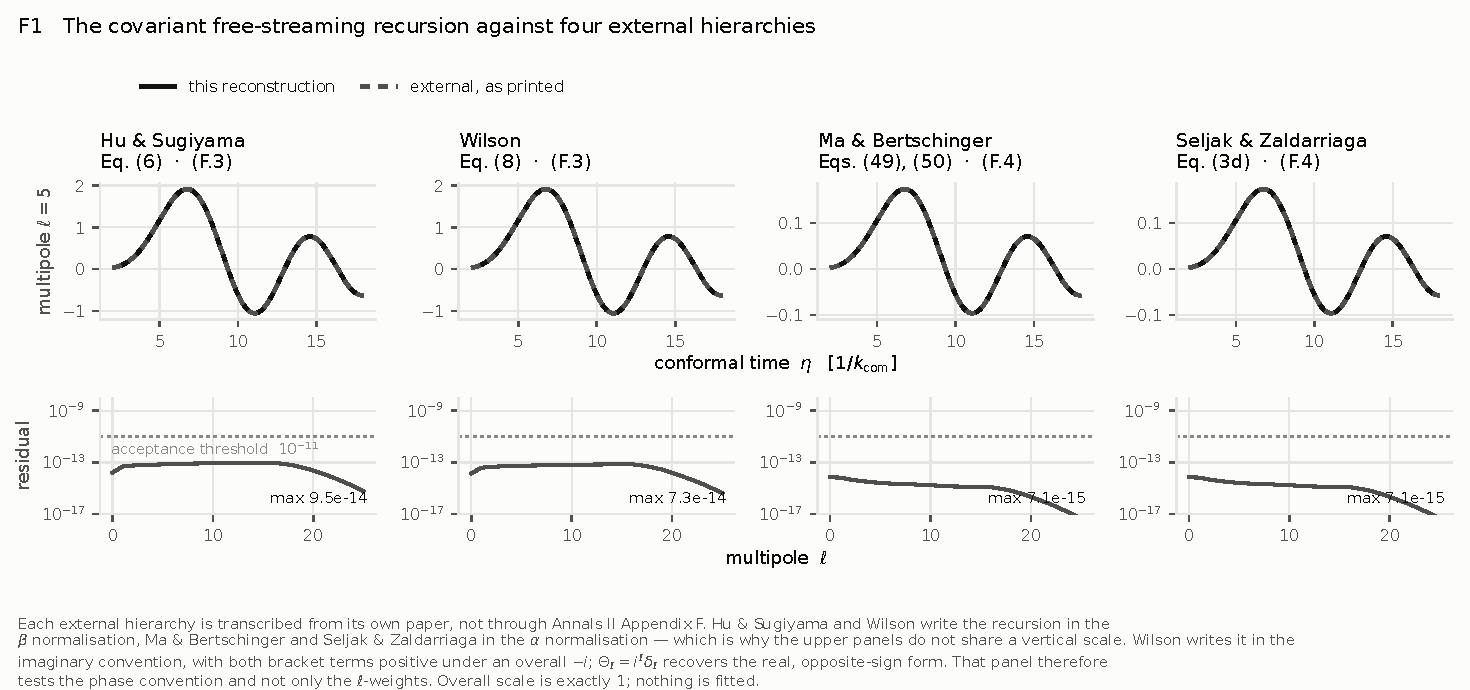
\includegraphics[width=\textwidth]{figures/f1-appendix-f-v1.0.0.pdf}
\caption[The covariant free-streaming recursion against three external hierarchies]{\textbf{F1 --- The covariant free-streaming recursion against three external hierarchies.} The covariant free-streaming recursion of \emph{Annals~II} Appendix~F, integrated from a unit monopole, against three external treatments of the same hierarchy. Each is transcribed from its own paper, never through Appendix~F. \textbf{Upper panels, context:} the reconstruction and the external form at $\ell=5$; they coincide. The panels do \emph{not} share a vertical scale, because two normalisations are on display. \textbf{Lower panels, the claim:} $\max_\eta|\mathrm{external}-\mathrm{reconstruction}|$ against $\ell$, with the acceptance threshold marked. Hu \& Sugiyama write the recursion in the $\beta$ normalisation and Ma \& Bertschinger and Seljak \& Zaldarriaga in the $\alpha$ normalisation, which is why Appendix~F prints both (F.3) and (F.4); a basis phase leaking into the couplings would break at least one match. Overall scale is exactly $1.000000000$ --- nothing is fitted. Three panels, not four: Wilson is pre-arXiv and the citation is ambiguous.\\[2pt]\footnotesize\emph{Evidence category:} cross-check. \emph{Generated by} \texttt{scripts/figure\_f1\_appendix\_f.py}. \emph{Standalone caption:} \texttt{captions/F1-appendix-f.md}.}
\label{fig:f1}
\end{figure}

\noindent\textit{Outstanding at this release candidate:} \textbf{F2} truncation convergence, both frames; \textbf{F3} angular autocorrelation; \textbf{F4} real-space angular correlation; \textbf{F5} source decomposition, two frames; \textbf{F6} impact of the approximations; \textbf{F7} frame specialisation; \textbf{F8} coupling schematic. The agreed specification for the full set is \texttt{captions/FIGURE-PLAN-v1.0.0.md}.
